\definecolor{osouter}{RGB}{235, 226, 192}
\definecolor{oslibs}{RGB}{238, 224, 145}
\definecolor{oskernel}{RGB}{239, 180, 141}
\definecolor{oshw}{RGB}{255, 110, 0}
\definecolor{ostext}{RGB}{25, 25, 25}

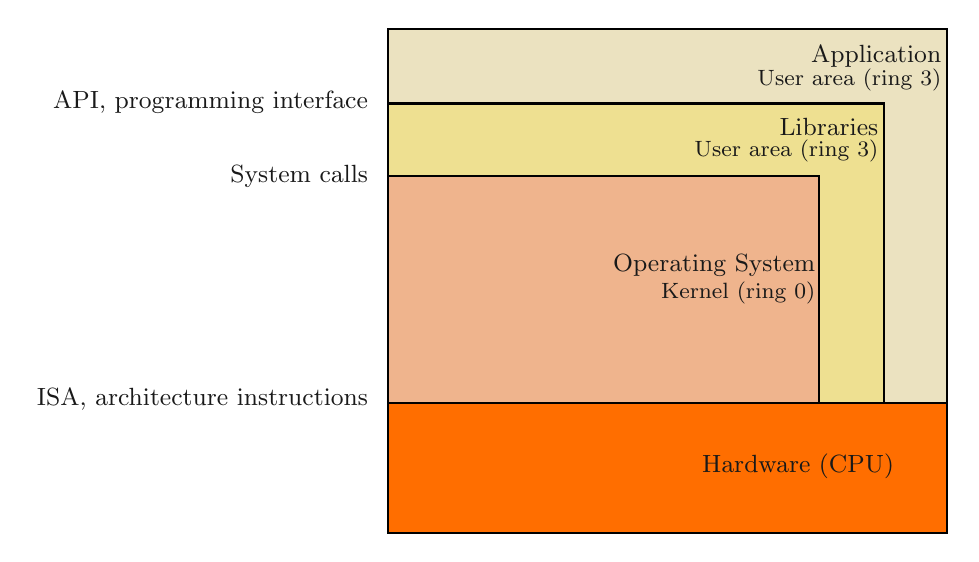
\begin{tikzpicture}[
  x=1cm,
  y=1cm,
  box/.style={draw=black, line width=0.8pt},
  biglabel/.style={font=\fontfamily{Inter-LF}\fontsize{9}{10}\selectfont, text=ostext},
  ringlabel/.style={font=\fontfamily{Inter-LF}\itshape\fontsize{8}{9}\selectfont, text=ostext},
  leftlabel/.style={font=\fontfamily{Inter-LF}\fontsize{9}{10}\selectfont, text=ostext, anchor=east}
]

  % Main stacked architecture
  \fill[osouter] (3.95, 0.45) rectangle (11.05, 6.85);
  \draw[box] (3.95, 0.45) rectangle (11.05, 6.85);

  \fill[oslibs] (3.95, 2.10) rectangle (10.25, 5.90);
  \draw[box] (3.95, 2.10) rectangle (10.25, 5.90);

  \fill[oskernel] (3.95, 2.10) rectangle (9.42, 4.98);
  \draw[box] (3.95, 2.10) rectangle (9.42, 4.98);

  \fill[oshw] (3.95, 0.45) rectangle (11.05, 2.10);
  \draw[box] (3.95, 0.45) rectangle (11.05, 2.10);

  % Left-side annotations
  \node[leftlabel] at (3.82, 5.92) {API, programming interface};
  \node[leftlabel] at (3.82, 4.98) {System calls};
  \node[leftlabel] at (3.82, 2.15) {ISA, architecture instructions};

  % Outer user area / application
  \node[biglabel, anchor=east] at (11.1, 6.5) {Application};
  \node[ringlabel, anchor=east] at (11.1, 6.20) {User area (ring 3)};

  % Libraries
  \node[biglabel, anchor=east] at (10.3, 5.6) {Libraries};
  \node[ringlabel, anchor=east] at (10.3, 5.3) {User area (ring 3)};

  % Kernel
  \node[biglabel, anchor=east] at (9.5, 3.85) {Operating System};
  \node[ringlabel, anchor=east] at (9.5, 3.50) {Kernel (ring 0)};

  % Hardware
  \node[biglabel, anchor=east] at (10.5, 1.30) {Hardware (CPU)};

\end{tikzpicture}
